\chapter{Question 4}
\label{available-representation}

\textbf{Choose your (the real you, not the substitute you) favorite and least favorite film from the data.  For each film, generate a list of the top 5 most correlated and bottom 5 least correlated films. Based on your knowledge of the resulting films, do you agree with the results?  In other words, do you personally like / dislike the resulting films?}

Following are the steps I have taken to solve the problem:

\begin{itemize}
\item I selected my favorite film as `Lion King (1994)' Movie\textunderscore Id `771' and least favorite movie as ` Johnny Mnemonic (1995)' with Movie\textunderscore Id `71'.
\item To get the top 5 most correlated movies and bottom 5 least correlated movies I have used the function calculateSimilarItems() from recommendations.py.
\item This is illustrated in the Listing \ref{lst:q4code1}
\item The output for this function is in the Figure \ref{fig:q4fig1}
\begin{figure}[h!]
\begin{center}
\hspace*{-3cm} 
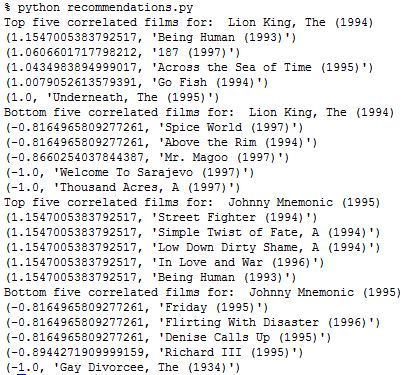
\includegraphics[scale=0.55, keepaspectratio=true]{figures/1.JPG}
\caption{Output with top 5 most correlated and bottom 5 least correlated movies for my most favorite and least favorite movie}
\label{fig:q4fig1}
\end{center}
\end{figure}
\item I personally like `Being Human (1993)' and `Across the Sea of Time (1995)' movies. I did not see the other 3 movies, I read the  summary in Wikipedia and IMDb, I liked `187 (1997)' , `Underneath, The (1995)' but I did not like `Go Fish (1994)'.
\end {itemize}


\newpage
\textbf{Code Listing}
\sloppy
\lstinputlisting[language=Python,caption=Function for getting top 5 correlated movies and bottom 5 correlated movies for my favorite and least favorite movies.,frame=single,breaklines=true,label=lst:q4code1, tabsize=2, captionpos=b,numbers=left,showspaces=false,showstringspaces=false,basicstyle=\footnotesize]{src/getRecommendations.py}